\chapter{State of the Art}
\section{Censorship Mechanisms}

The following section is based primarily on information from the source \textit{RFC 9505
A Survey of Worldwide Censorship Techniques} \cite{rfc9505}. Any other information sourced from elsewhere is identified as such.

\subsection{IP Blocking}

Internet Protocol (IP) blocking is one of the most straightforward censorship techniques. Each device connected to the internet is assigned a unique numeric label called an IP Address, which serves as an identifier that allows data to travel across the internet to the correct destination. When a government or ISP wants to censor a specific website it can be implemented in either incoming or outgoing traffic. ISP controlled firewalls can be configured so that any outgoing or incoming requests to a selected IP address are dropped. ISPs can also adjust routing tables in their network to remove an IP address, making it unreachable for the user. 

IP blocking can either be implemented at a centralized level or at an ISP level. In Ireland, IP blocking is done at an ISP level to block certain illegal websites in accordance with court orders (see section 2.2 for more information). In Iraq, IP blocking is implemented at the ISP level under the directive of the Ministry of Communications \cite{freedomhouseIraqFreedom} (see section 2.3 for more details).

\subsection{DNS Blocking}

DNS blocking refers to the altering of responses from the DNS to block or filter access to certain content. This is usually done by either blocking the response, replying with an error message, or responding with an incorrect address. \textit{DNS Mangling} is a network-level technique of on-path interception where an incorrect IP address is returned in response to a DNS query to a censored destination. 

\textit{DNS Cache Poisoning} is an off-path technique in which a censor intercepts and replaces the legitimate response from an authoritative DNS name server with a spoofed IP address. Instead of allowing the real IP address of a site to reach the user, the censor replies faster than the real server, and that spoofed IP gets cached (perhaps by numerous recursive resolvers). Subsequent requests will then be redirected to an incorrect IP, normally leading to a warning page or a meaningless domain. In other cases, such as in Iran, the censor can merely block the response of the upstream resolver, so the accurate IP address is never transmitted.

\textit{DNS Lying} is the most authoritative approach, where a censor mandates that the DNS responses provided are to be different from what would actually be returned by the DNS server \cite{rfc9505}.

(add more detail)

\subsection{Deep Packet Inspection (DPI)}

Deep Packet Inspection consists of any kind of packet analysis beyond IP address and port number. DPI reassembles network flows to examine the application data section, and is often implemented using Middleboxes. DPI is often used for keyword identification, but this method can also determine packet size and flow timings to detect other forms of content, such as the difference between text or video packets. Although DPI has difficulty with encrypted data and is the most expensive form of censorship to implement, it is still the most powerful identification method and is widely used in practice \cite{rfc9505}.

\subsection{Transport Layer Security (TLS)}

Transport Layer Security (TLS) may be censored by mechanisms similar to those against plain HTTP, particularly through the Server Name Indication (SNI) field. In the case of TLS over TCP, the SNI value is seen in the non-encrypted ClientHello message so that censors can inspect the field and exclude connections to those domains they disapprove of. While QUIC encrypts ClientHello, the initial encryption keys are visible to network observers, and therefore it is possible, though more complex, to decrypt and observe the SNI. Since 2018, the governments of China, Egypt, Iran, Qatar, South Korea, Turkey, Turkmenistan, and the United Arab Emirates have implemented widespread SNI filtering or blocking \cite{rfc9505SNIBlocking}. 

Attempts to encrypt SNI have resulted in Encrypted SNI (ESNI), which embeds the SNI field in encrypted traffic but can induce blanket blocking by censors who blindly terminate all ESNI connections. Even more comprehensive security improvements, such as Encrypted Client Hello (ECH) for TLS 1.3, aim to encrypt the whole ClientHello rather than merely the SNI, though these enhancements are still underway in standardization and deployment.

Another way is to not include the SNI at all. However, non-SNI connections can be blocked as well, since censors can deploy policies that will drop any TLS traffic that does not have an SNI. This can again lead to overblocking, since clients that are able to handle older SSL-only configurations, or are deliberately configured not to have an SNI, can get blocked even when they are going to otherwise acceptable sites.

Censors also have the option to examine the server certificate field within the TLS handshake, which contains information on the requested domain. In TLS 1.3, however, certificates are encrypted by default, and thus such censorship is not possible. Certificate-inspecting censors must therefore employ more computation-intensive deep packet inspection techniques and can even be forced to track connections deeper into the handshake process, especially when SNI-based approaches fail or bypassed \cite{rfc9505}.

\subsection{Network Blackouts}

\subsection{TEMP NAME TABLE}

\begin{table}[h!]
\centering
\begin{tabular}{ |p{3cm}|p{3cm}|p{3cm}|  }
\hline
Censorship Mechanism & Ireland & Iraq \\
\hline
Afghanistan & AF &AFG \\
Aland Islands & AX   & ALA \\
Albania &AL & ALB \\
Algeria    &DZ & DZA \\
American Samoa & AS & ASM \\
Andorra & AD & AND   \\
Angola & AO & AGO \\
\hline
\end{tabular}
\end{table}

\section{Ireland}

\subsection{Censorship in the Past}

According to a report from the United States Department of State in 2011, it was found that there were no government restrictions on access to the internet or that the government actively monitored email or internet chatrooms \cite{stateTechnicalDifficulties}.

The Irish government engages in censoring or blocking the distribution of pirated copryrighted material. In 2009, the Irish Telecom Company, EIRCOM, blocked its customers from accessing the website \textit{The Pirate Bay}. The Pirate Bay is a Swedish website which provides links to copyrighted material. The website was hit with a lawsuit from major record labels and many ISPs around the world agreed to block access to the website as part of the settlement. However, not all Irish ISPs complied. The cable TV operator UPC announced that it would not comply \cite{irishtimesEircomBlock}. 

In alignment with international agreements, the Irish Government blocks access to websites that contain illegal content, such as Child Sexual Abuse Material (CSAM). The government has setup a hotline that allows citizens to anonymously report websites that they suspect contain illegal content, called hotline.ie \cite{hotlineAboutx2013}.

In contrast to other EU countries, Ireland does not have a broad government-mandated filtering system. They instead have the power through the Irish courts to mandate Irish ISPs to block certain websites. In addition, Irish ISPs may voluntarily enforce content filtering and website blocking in alignment with Irish content law.

Up until 2014, Ireland and other EU countries followed data retention laws, which required ISPs to store metadata for law enforcement purposes. In 2014, the European Court of Justice struck down the directive, which led to a change in this law in Ireland \cite{DataRetentionInvalid2014}. After this change, Ireland enacted the \textit{Communications (Retention of Data)(Amendment) Act 2022} \cite{irishlegalDataRetention}. This legislation allows for the general and indiscriminate retention of communications traffic and location data on the grounds of national security, where approved by a judge.

\subsection{Current Censorship}

As a whole, Ireland's censorship efforts are limited and specific. The government and ISPs target mainly illegal and pirated content. Some specific websites that have been blocked include 1337x, Eztv, BMovies, GoMovies, Putlocker, Rarbg, WatchFree, and Yts \cite{siliconrepublicMovieIndustry}. However, piracy websites are still widely accessible in Ireland.

It seems that Ireland has also rolled back blocks on some websites, such as Russian News outlets. Previously, the domain russia.tv, was blocked in Ireland. But as of 2025, it is able to be partially accessed. Based on data from the OONI project, there is evidence of TCP/IP blocking of this domain in Ireland. Based on the findings from OONI, this domain is able to be accessed when EIRCOM's root DNS server (AS5466, IP: 86.47.80.38) is used, but is blocked when accessed through Cloudflare's DNS server (AS14593, IP: 172.69.193.80).

\centerline{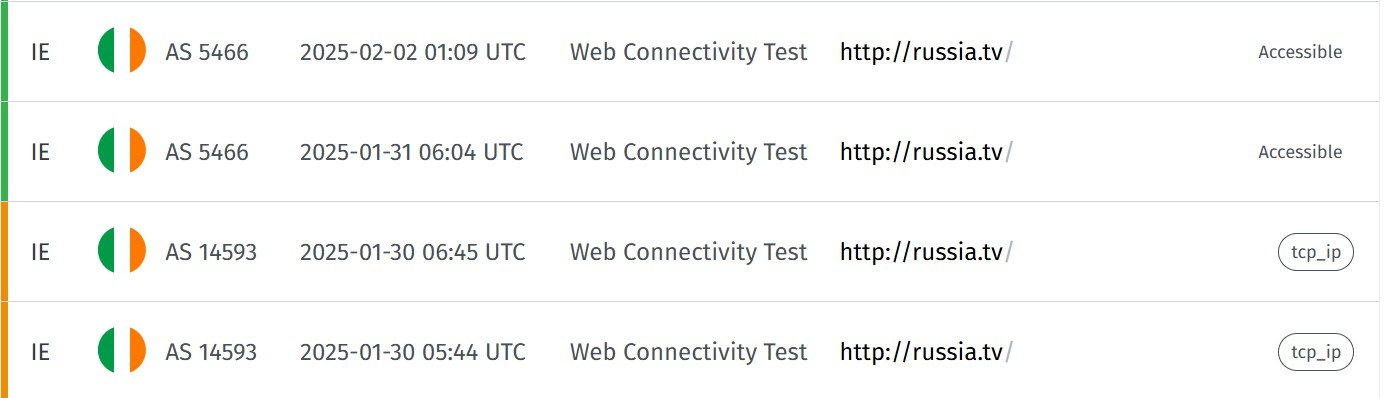
\includegraphics[width=480pt]{Griff/Latex/TCD SCSS CAPSTONE/Literature Review/RussiaTV search OONI.jpg}}

\centerline{\textit{Figure 1.3, Russia.tv domain search on OONI}}

\section{Iraq}

\subsection{Censorship in the Past}

Iraqi internet censorship has been radically reshaped over the years. Under Saddam Hussein's regime, only a very few Iraqis had access to the internet, leading to the state controlling all parts of the internet within the country. Post-2003, with more people accessing the internet and the country struggling with internal conflict and the threat of radicalization, censorship was decentralized and usually carried out with little transparency and regionally differentiated. While the constitution and laws of Iraq recognize free expression, actual enforcement is usually slow whenever security is at stake. As the internet began to take a greater role, both as a platform for political discourse and a vehicle for extremist messaging, the censorship and intrusions of the government increased correspondingly. Generally speaking, the policy of controlling the internet in Iraq has mirrored the broader political and security situation, tightening whenever Iraq is unstable \cite{freedomhouseIraqFreedom}.

\subsection{Current Censorship}

Iraq's internet growth progressed from state-controlled limitations during Saddam Hussein's era, where limited citizens used the internet. After 2003, many private ISPs were formed, but primary fiber routes and gateways that link Iraq to international submarine cable networks via adjacent countries are still controlled by the Ministry of Communications \cite{IraqCMC}. Baghdad, the country's capital and commercial center, is a hub of national connectivity, and other large cities (like Basra and Mosul) typically have local backbones that connect into the national fiber network. The Kurdistan Region of Iraq (KRI) also has standalone network configurations, with cross-border fiber routes—particularly to Turkey—creating a semi-independent internet ecosystem \cite{freedomhouseIraqFreedom}. 

In a 2023 report from the United States Department of State, it was found that the government of Iraq restricted or disrupted access to the internet and censored online content, in conjunction with monitoring private online communications without appropriate legal authority \cite{USDoSIraq2023}. The Iraqi government and the Kurdistan Regional Government (KRG) consistently engage in implementing internet outages during protests or times of unrest \cite{freedomhouseIraqFreedom}. In 2023, Iraqi officials implemented 66 internet outages, more than any other country in the world. 

After the fall off Saddam Hussein's Regime in 2003, the internet became much more accessible and the information landscape was opened. However, the current-day Iraqi government occasionally blocks websites, and more often social media websites in order to maintain stability and control during times of unrest \cite{freedomhouseIraqFreedom}. During anti-government protests in 2019, the Iraqi government blocked access to Facebook, X (Formerly Twitter), WhatsApp, and Instagram. In protests in 2018, some users in Iraq found that they were unable to use VPNs to circumvent website blocking. The government routinely engages in the censoring and blocking of Pornography and Gambling websites on the guise of protecting their citizens from harmful content. 

\section{Censorship Circumvention Tools}

\subsection{The Tor Browser}

\subsubsection{The Tor Project Background}

The Tor Browser is built on a concept called \textit{Onion Routing}, which was developed in the 1990s by researchers at the United States Naval Research Laboratory. The goal of the project was to create a communication method where data is wrapped in multiple layers of encryption so that no point in the network could reveal the sender and receiver \cite{torprojectProjectPrivacy}. Originally, the United States Government used the Tor network to access potentially illegal websites anonymously, and transmit data. But because only the US Government was using it at the time, it was easy to tell who the single anonymous user was, when viewing the site logs. It would also have made Tor a target for bad actors, as they could be sure that all data being sent over the network was related to the United States Government/Military.

To stop this from happening, the US Government released Tor to the public in the early 2000s, and later it became the Tor Project, a non-profit organization funded by the United States that develops and maintains the Tor software. 

\subsubsection{Technical \& Circumvention Information}

Internet traffic sent over the Tor network is encapsulated in multiple layers of encryption. Think of your data as a letter that is placed inside several envelopes. Each node in the network removes one envelope, revealing only the information necessary to pass the message along to the next node. To do this, the Tor browsers sends your data through at least three nodes, and the pathway of these nodes are randomly constructed and reconstructed during your session \cite{dingledine2004tor}.

\centerline{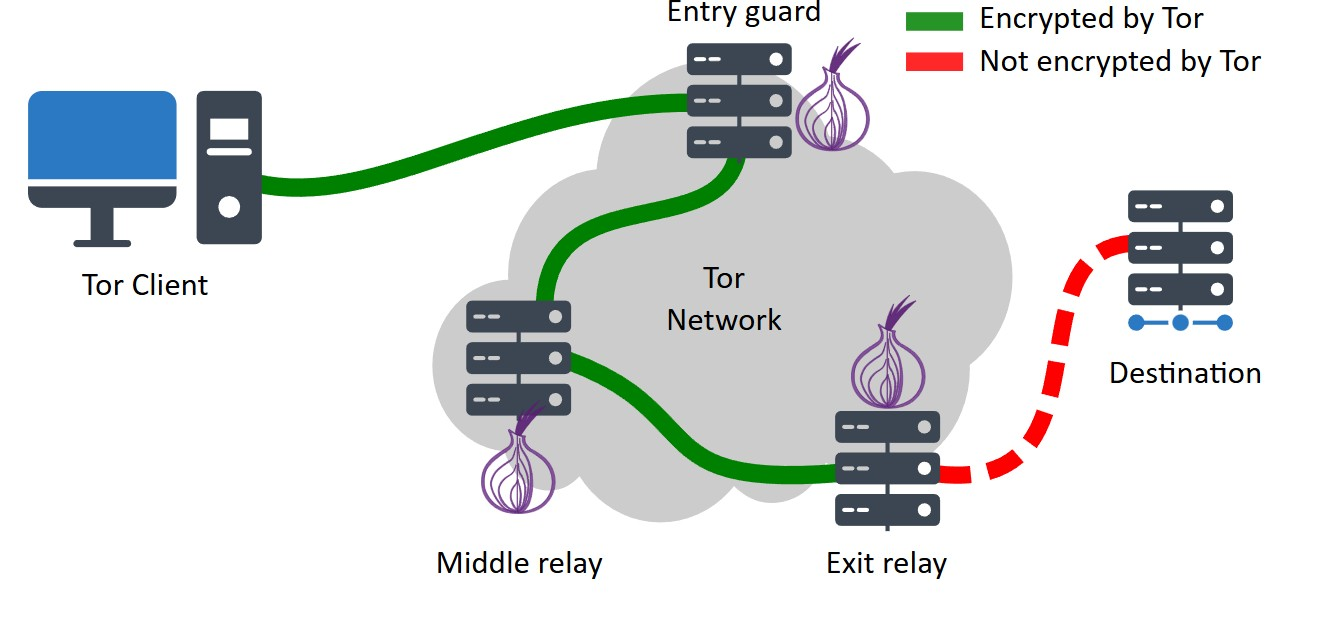
\includegraphics[width=480pt]{Griff/Latex/TCD SCSS CAPSTONE/Literature Review/How tor works.jpg}}

\centerline{\textit{Figure 1.4, How the Tor Network Works}}

Tor is a great tool to combat censorship. Tor's distributed architecture of nodes makes it resilient against localized censorship efforts. In countries where the Tor network is blocked, users are able to use "Bridges", which are Tor nodes that are not listed publicly. Using a bridge address allows for the user to connect to the network covertly \cite{torprojectBRIDGESProject}. Users can also avail of "Pluggable transports", which transforms Tor traffic to look like regular network traffic. This method can help circumvent censorship in regions that use \textit{Deep Packet Inspection} (DPI) and other forms of advanced internet censorship \cite{torprojectCIRCUMVENTIONProject}.

\subsection{VPNs}

Virtual Private Networks (VPNs) broadly speaking provide an end-to-end encrypted connection between your device and a VPN server. This method hides your IP address and grants the user anonymity while browsing over the network. This allows users to bypass censorship by connecting to servers outside of their location while masking your IP address \cite{TomsGuideVPN}. 